\documentclass{beamer}
\usepackage{graphicx}
\title{Cooperative Strategies in Multi-Agent Systems}
\author{James King}
\usetheme{metropolis}
% Purpose of presentation:
%% Explain the aims and objectives clearly
%%% Explore the mechanism of indirect reciprocity's relevance to multi-agent systems and the application of various strategies within the same game
%% Explain the background/relevance/importance of the project in a wider context
%%% Natural Selection
%%% Relevance to agent systems
%%% Iterated Prisoner's dilemma
%% Broad description of the project
%% Theory underpinning parts of the project
%% Communicate well, support with a clear simple presentation
%% Defend and justify decisions
\begin{document}
	\frame{\titlepage}
	\frame{
		\frametitle{Outline}
		\tableofcontents
	}
	\subsection{The Problem}
	\frame{
		\frametitle{The Problem}
		\Large\center ``Survival of the fittest."\\ \center - Herbert Spencer in The principles of biology
	}
	\subsection{The Mechanism}
	\frame{
		\frametitle{The Mechanism}
		\begin{center}
			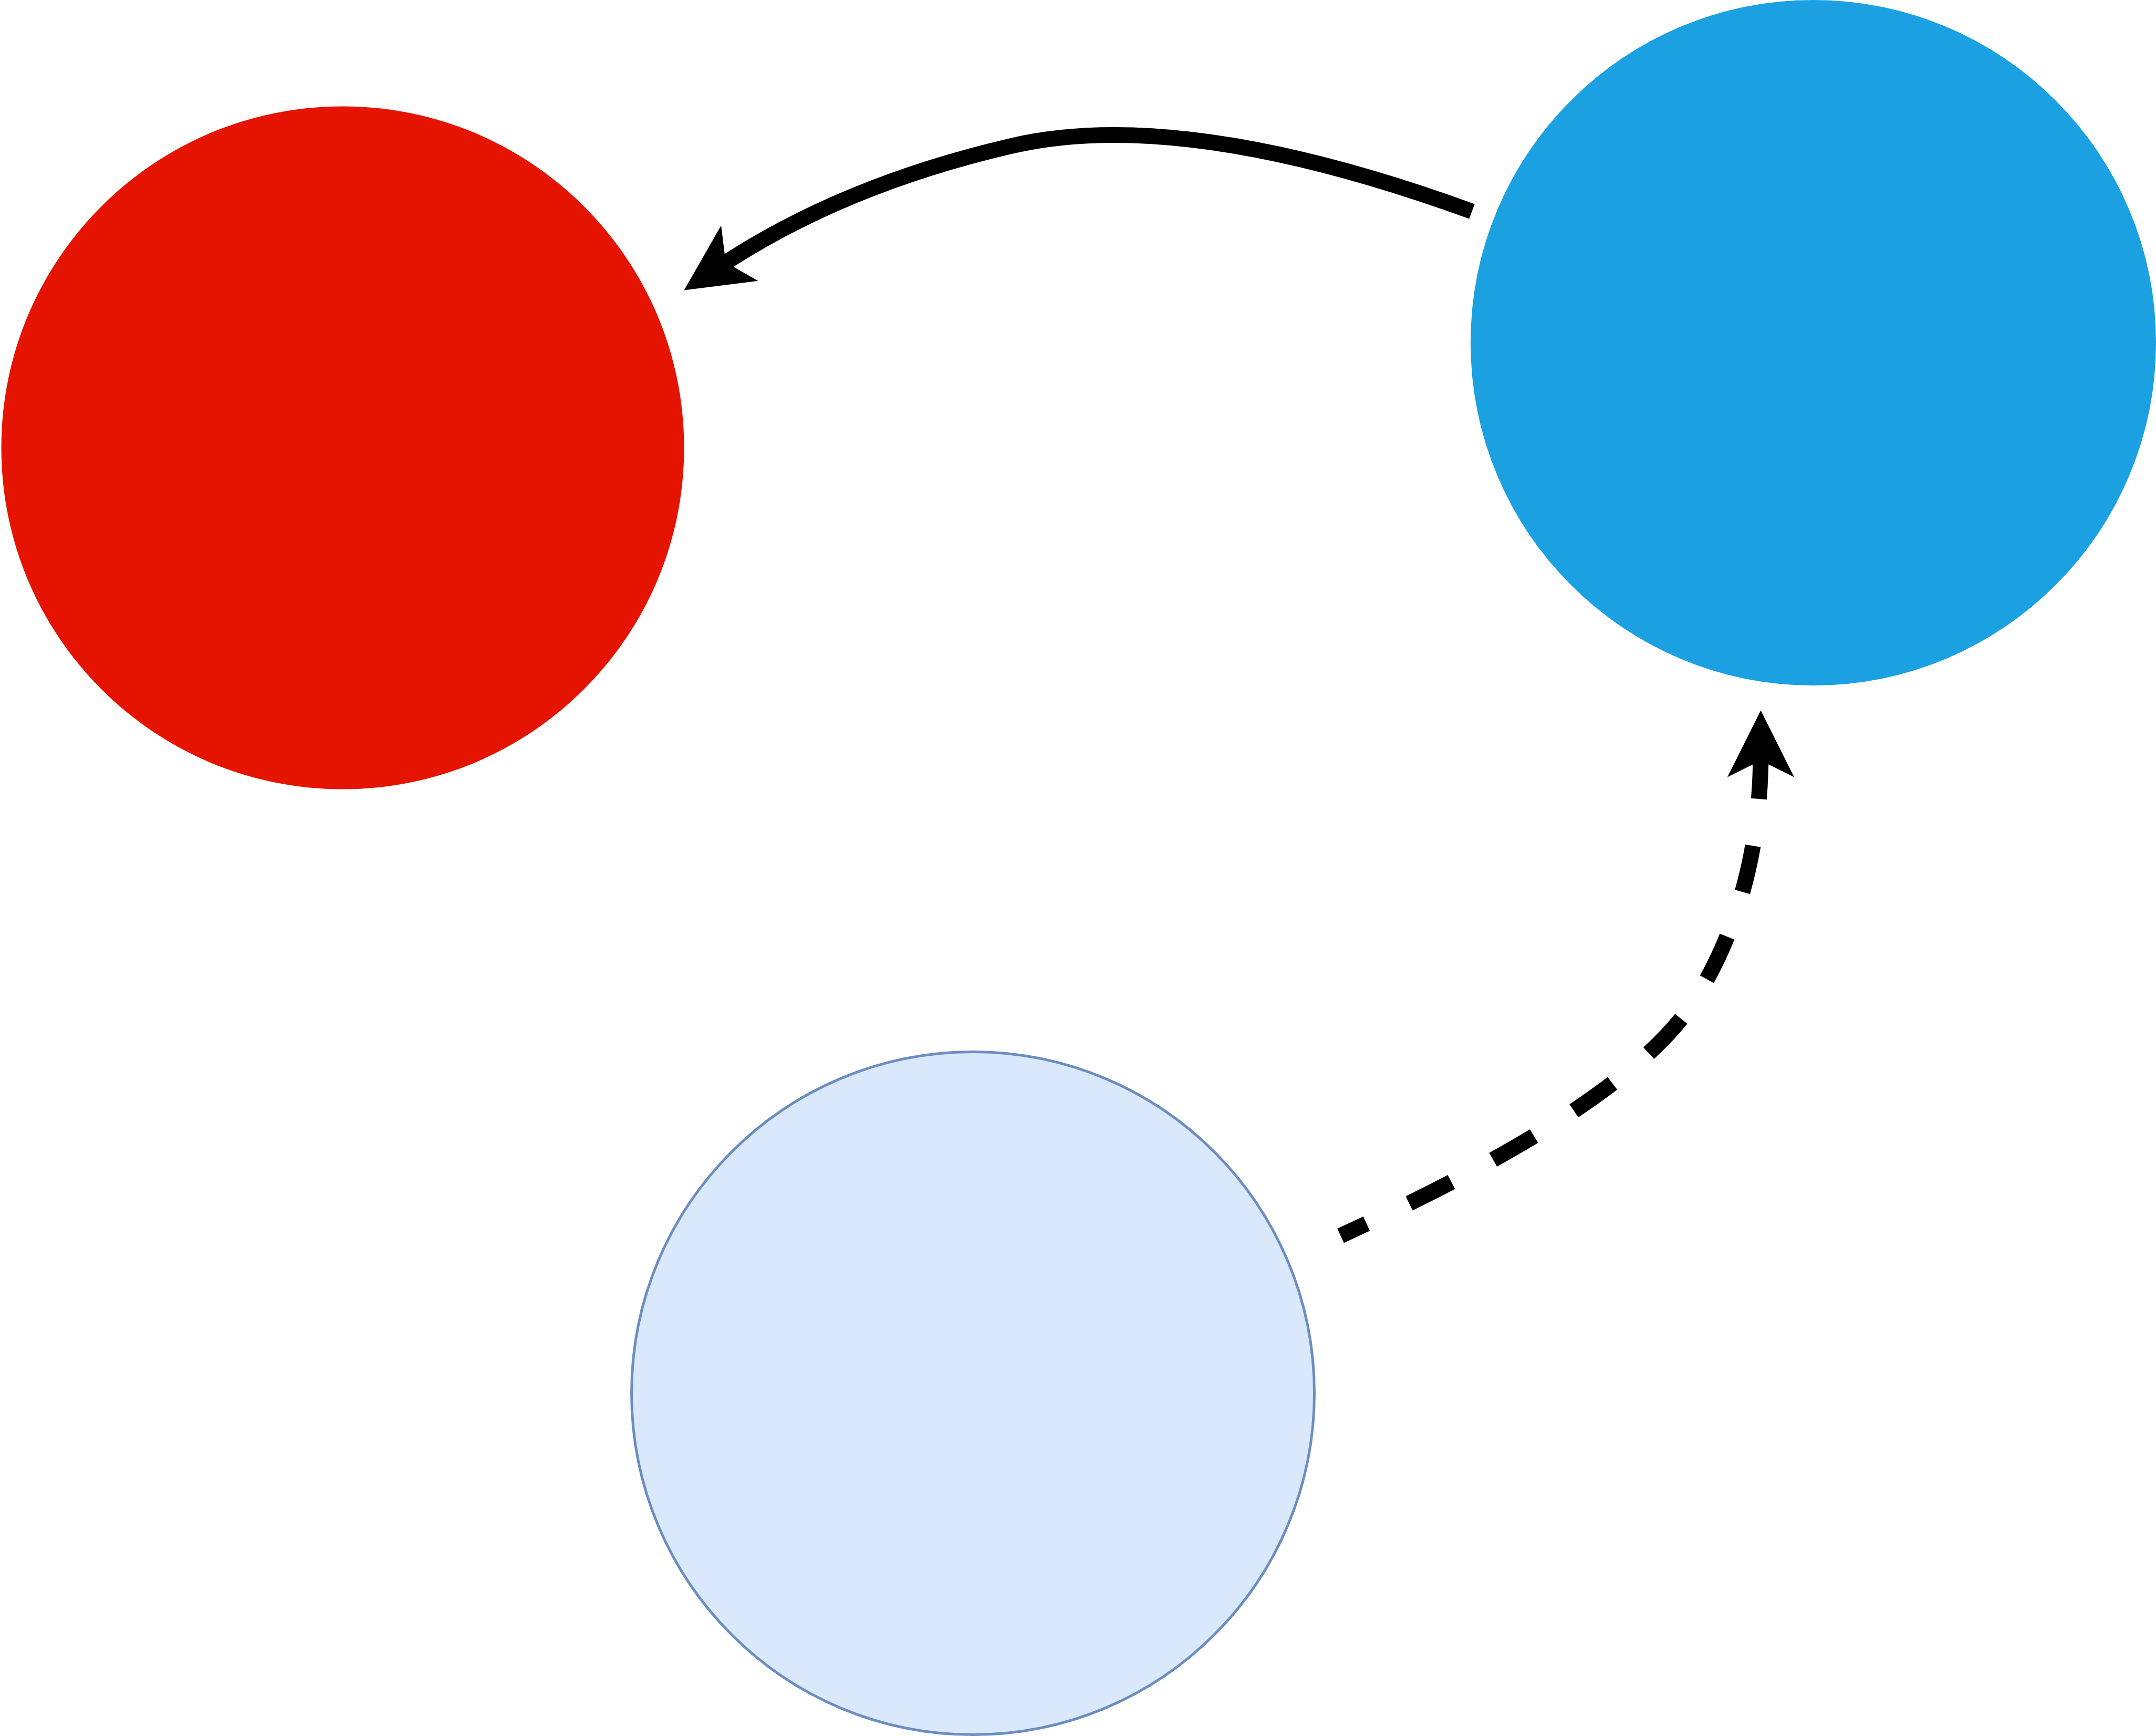
\includegraphics[height=0.7\textheight]{IndirectRec.png}
		\end{center}
		\footnotetext[0]{Taken from Nowak and Sigmund 1998~\cite{evol_indirect_image}}
	}
	\subsection{The Aims and Objectives}
	\frame{
		\frametitle{The Aims and Objectives}
		\begin{itemize}
			\item Explore the mechanism of indirect reciprocity's relevance to multi-agent systems
			\item Explore different strategies success in the game
			\item Explore different trust models for agents in a multi-agent system
			\item Explore how social ability can affect the evolution of cooperation in a system
		\end{itemize}
	}
	\subsection{The Implementation}
	\frame{
		\frametitle{The Implementation}
		\begin{center}
			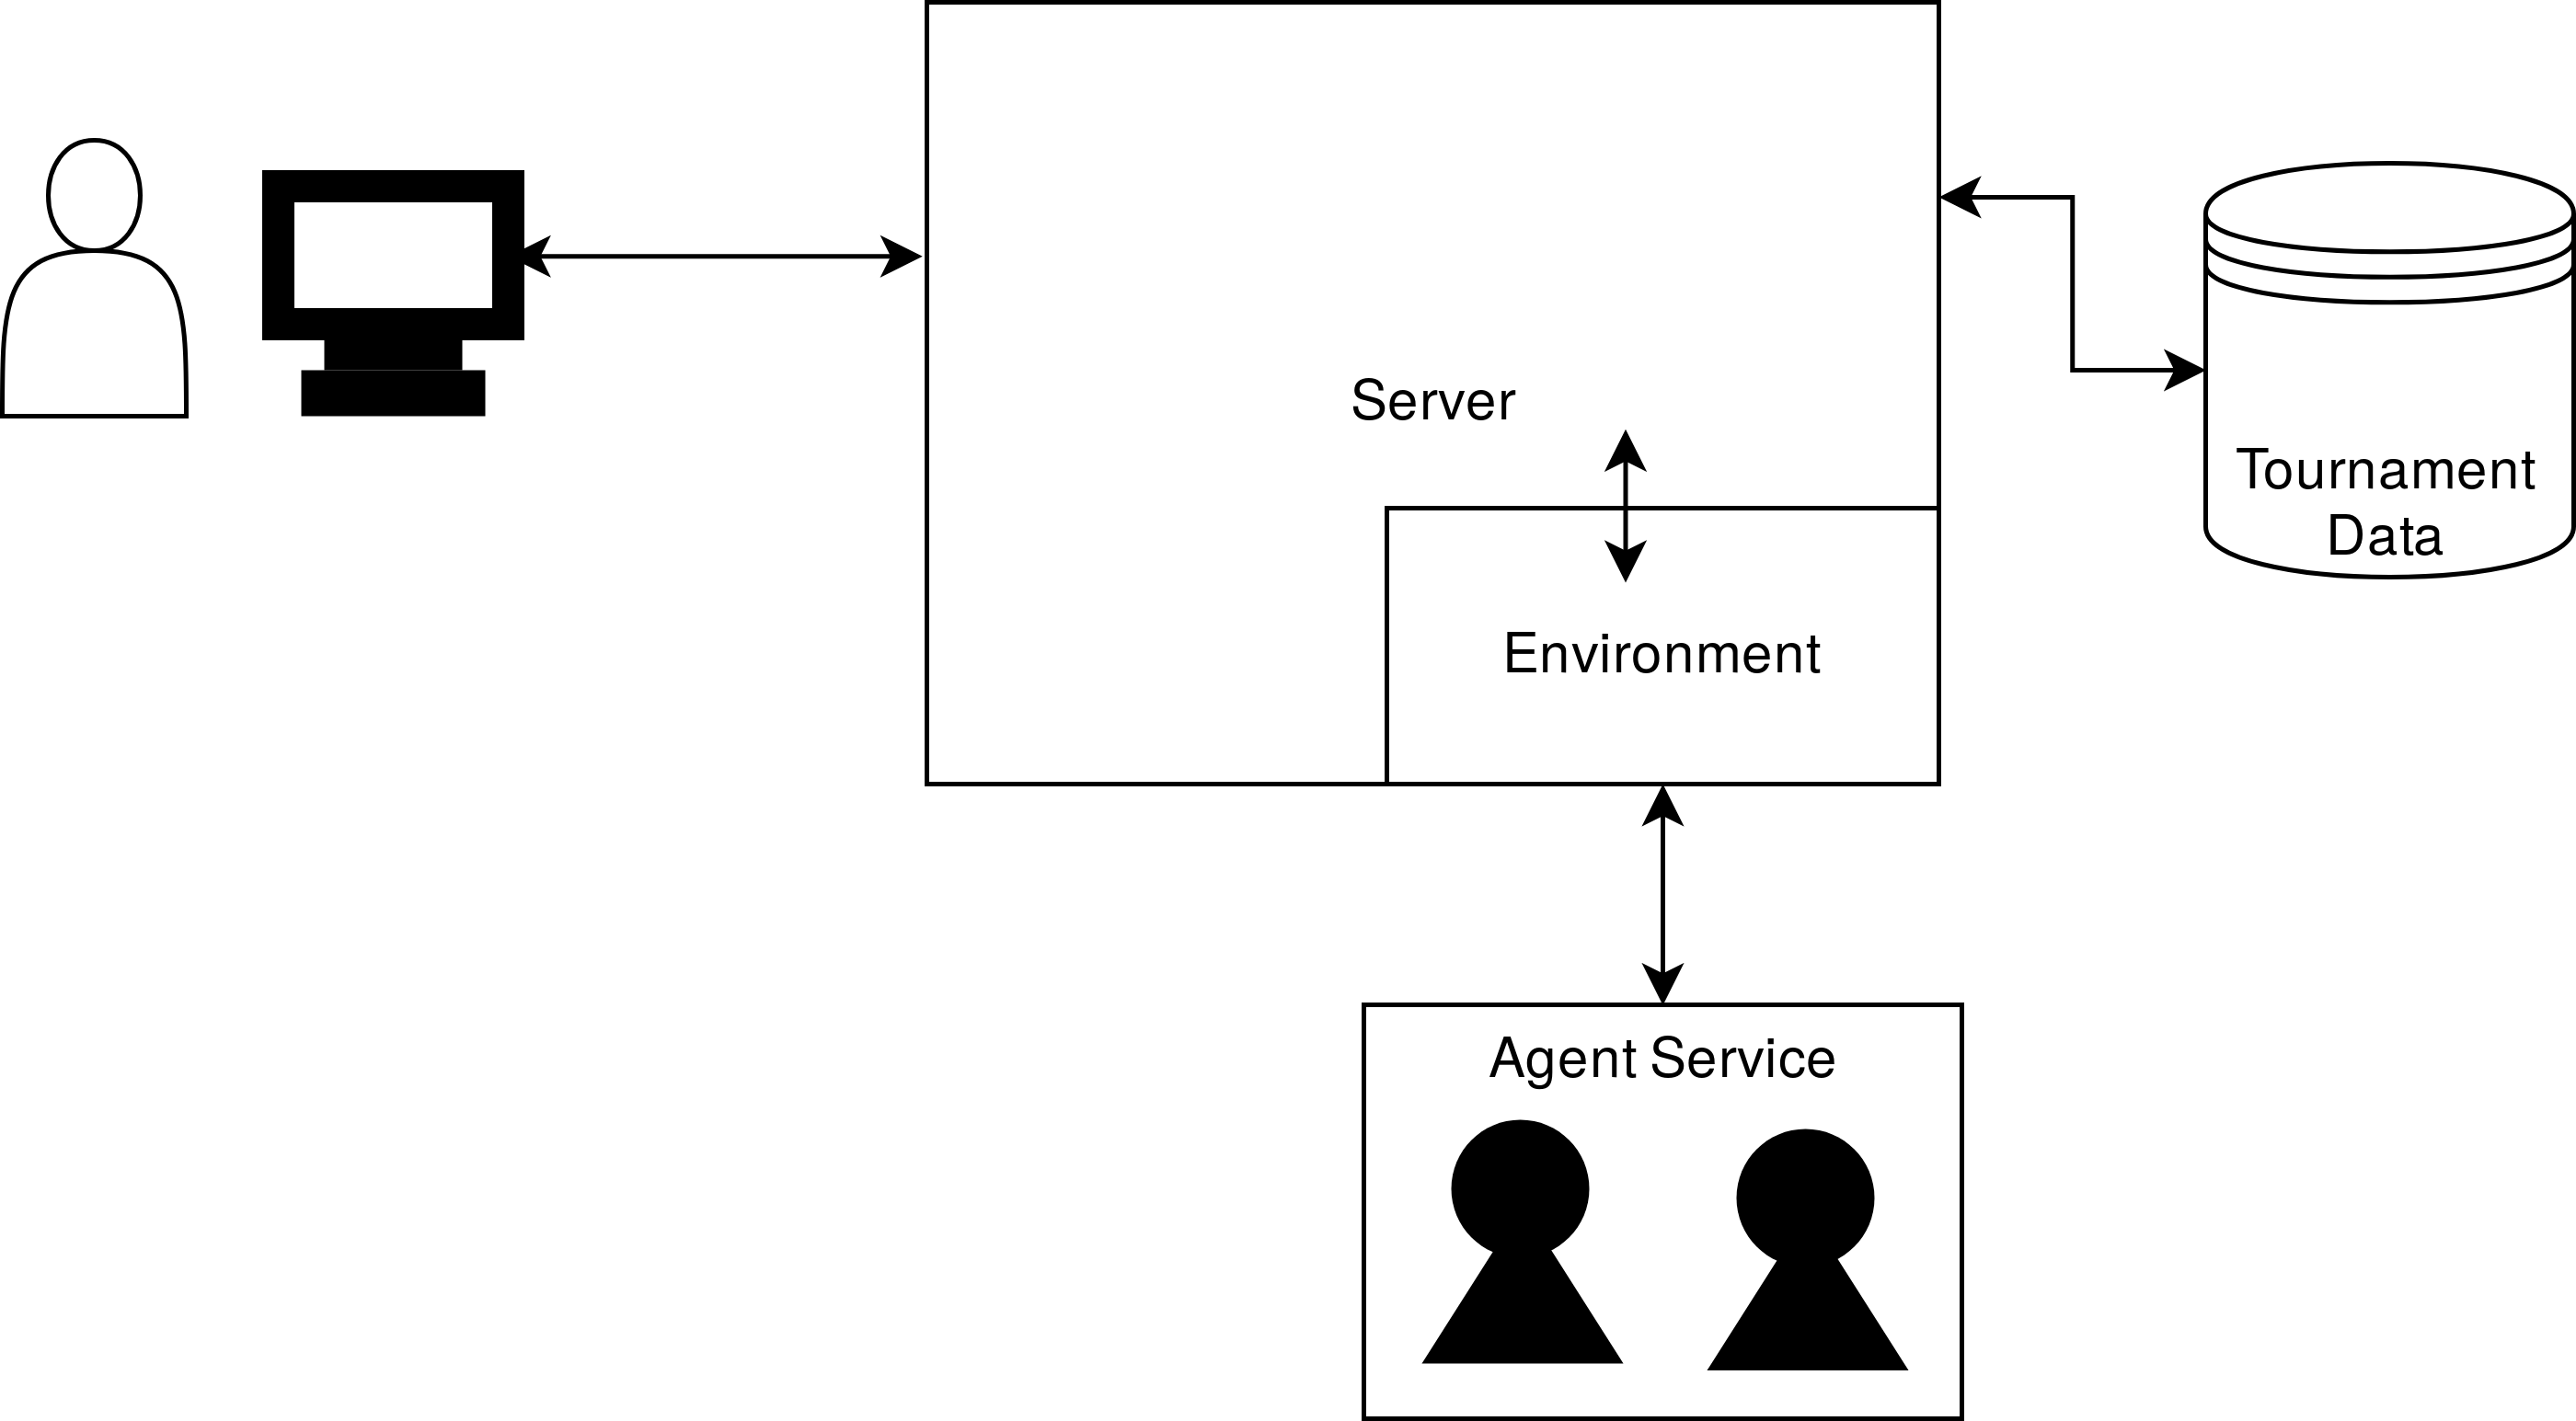
\includegraphics[width=1\textwidth]{PresSystem.png}
		\end{center}
	}
	\subsection{The Future}{
	\frame{
		\frametitle{The Future}
		\begin{itemize}
			\item Improving the environment class structure and testing
			\item Post-tournament analysis
			\item Front-end for an indirect reciprocity game
			\item Expanding the API
			\item Developing more agent strategies
			\item Improving agent proactivity
			\item Making the web application design fit for education (enhanced GUI + content)
			\item Development of a learning agent
		\end{itemize}
	} 
	\frame{
		\frametitle{Bibliography}
		\bibliography{../refs.bib}{}
		\bibliographystyle{plain}
	}
\end{document}